\documentclass[twocolumn, a4paper, 9pt]{UECIEresume}

\usepackage[dvipdfmx]{graphicx}
\usepackage{graphicx}
\usepackage{amsmath}
\usepackage{txfonts}
\usepackage{epsfig}
\usepackage{tabularx}
\usepackage{amssymb}
\usepackage{url}
\usepackage{mediabb}
\newcommand{\bhline}{\noalign{\hrule height 1pt}}
\newcommand{\ab}{\allowbreak}

\title{Twitterを用いた携帯端末における個人認証の多要素化に関する研究}
\date{平成 26 年 02 月 10 日}
\affiliation{総合情報学科 セキュリティ情報学 コース}
\supervisor{高田 哲司 准教授}
\studentid{1010086}
\author{高浪 悟}
%\headtitle{平成 yy 年度 総合情報学科 卒業論文中間発表}
\headtitle{平成 25 年度 総合情報学科 卒業論文発表}
%\headtitle{平成 yy 年度 総合情報学科 修士論文中間発表}
%\headtitle{平成 yy 年度 総合情報学科 修士論文発表}

\begin{document}
\maketitle

\section{はじめに}
高性能な携帯端末の普及により,個人や決済にかかわる重要な情報を持ち歩くことが一般化しつつあり,必然的に個人認証を行う場面が増えてきている.
こういった場面における個人認証では,パスワードや暗証番号(PIN\footnote{Personal Identification Number})を用いた例をよく見かける.

特にパスワードを用いた認証では,安全性と記憶持続性・利便性に関してはトレードオフの関係が存在する.
例えば,辞書攻撃に強い安全なパスワードを用いようとする際には,意味のない文字列にすることが望ましい.
しかし,意味のない文字列というのは覚えることが難しく,ユーザがパスワードを他のサービスにおいても使い回してしまう可能性が高まり,そうするとどれか一つのサービスからパスワードが流出した際,かえって脆弱になってしまう.
現在,こういった問題を防ぐものとして,多要素認証を利用できるWebサービス(Google,Facebookなど)が増加しつつある.
多要素認証の多くは,パスワードの入力が完了し,それが正しいものだと判断された後に,ユーザが特定の手法で入手したワンタイムパスワードを入力させるといった方式をとっており,覗き見,推測や総当り攻撃によってパスワードが漏洩した際の不正利用のリスクを減少させることが可能となる.
多要素認証を何らかの方法で適用する行為を個人認証の多要素化と定義する.

また,Social Networking Service\footnote{社会的ネットワークをインターネット上で構築するサービス.}(以下,SNS)の形態を持つWebサービスが近年増えてきており,コミュニケーションの道具やライフログとして自分自身の情報を公開することが多くのユーザ間で一般的になりつつある.
SNSにおいては,公開範囲をある程度任意に指定できるサービスが多いという特徴がある.

本研究における目的は,利便性に考慮しつつ個人認証の安全性を向上させることである.
現在行われている個人認証の多要素化は,セキュリティトークンやEメールを用いたものが一般的であり,それにより大きく認証の安全性を高めている.しかし,利便性という点においては,一度認証のための画面から目を逸らす必要がある,特別なハードウェアを持ち歩く必要があるなど,今後の普及に際して改善の余地があると考えられる.
また,近年普及しているSNS\cite{soumuWhitepaper2013Social}やライフログの情報を用いて利便性を損なわずに安全性を向上可能な認証システムを提案できないかと考えた.

\section{関連手法}
多要素認証を導入している代表的なWebサービスであるGoogleでは,アカウントを認証するための手段として,(1)SMSを用いてワンタイムパスワードを送信する方式,(2)音声通話によりワンタイムパスワードを確認する方式,(3)携帯端末向けアプリケーションでワンタイムパスワードを生成する方式,(4)バックアップコードを予め保存しておく方式,の4種類の多要素認証手法を用意している\cite{google}.

ライフログやWebサービスを認証に用いる手法に関して,西垣ら\cite{西垣正勝:2006-03-15}は,ユーザの生活履歴を用いて認証を行う手法を提案し,そのプロトタイプとしてEメールを用いたシステムの構築と実験を行った.Eメールによる認証は,「最近のメールかどうか」をユーザに回答させるというプロセスで行われた.その際,人間の記憶の曖昧性を取り除くための手法として,最近と過去どちらともいえないような期間のメールを利用しない,例えば「8日前から29日前までのメールは質問の中に出てきません」と明示することでユーザが直感的に回答を行えるようにした
また,Nemotoら\cite{nemoto:2006-03-15}は,Twitterのダイレクトメッセージ\footnote{特定のユーザ宛に,一対一で送信された文章のこと.閲覧可能な人物は,自分と相手のみである.}(DM)機能を用いて,定期的に質問を投げかけることでその回答を秘密情報とし,認証を行うシステムを提案した.
質問の内容は「2月15日の昼食は?」といった文面で構築され,Twitterのダイレクトメッセージ機能により送信され,回答も同機能を用いて行う.

\section{提案システム}
本研究における提案システムとして,以下の機能を持つ個人認証手法を実装した:
(1)利便性と安全性を両立させるために,SNS上に存在する情報を秘密情報として使用する
(2)手軽且つ環境へ依存せず導入し安全性を向上させることが可能な多要素認証のモデルケースとして,携帯端末における既存の知識認証に付け加わるように動作する

今回はライフログとしての性質を持つSNSとしてTwitterを用い,その中でも能動的な行為によって生成される情報である自分の投稿(ツイート)を秘密情報とした.
更に,携帯端末向けプラットフォームとして国内における利用率の高いiOSを選択した.

本研究では3種類の提案手法を用意した.

\subsection{Auto Mode Type Term}
図\ref{notifauthSettings}左のように,○日/週/月/年前から△日-年間を指定し,認証時点にその範囲に当てはまるツイートが秘密情報となり,それ以外が不正解の選択肢となる.
設定時もしくは前回の認証時から新しく投稿されたツイートも秘密情報の候補として含まれ,ツイートを選択した後は従来のPIN認証との比較のため4桁のPINを入力する.

\subsection{Auto Mode Type Cycle}
図\ref{notifauthSettings}右のように,○曜日の△時台という条件に当てはまるツイートが秘密情報となり,それ以外が不正解の選択肢となる.
新しく投稿されたツイートの扱いと認証の手順はAuto Mode Type Termに準ずる.

\begin{figure}[ht]
  \begin{minipage}{0.49\hsize}
    \begin{center}
      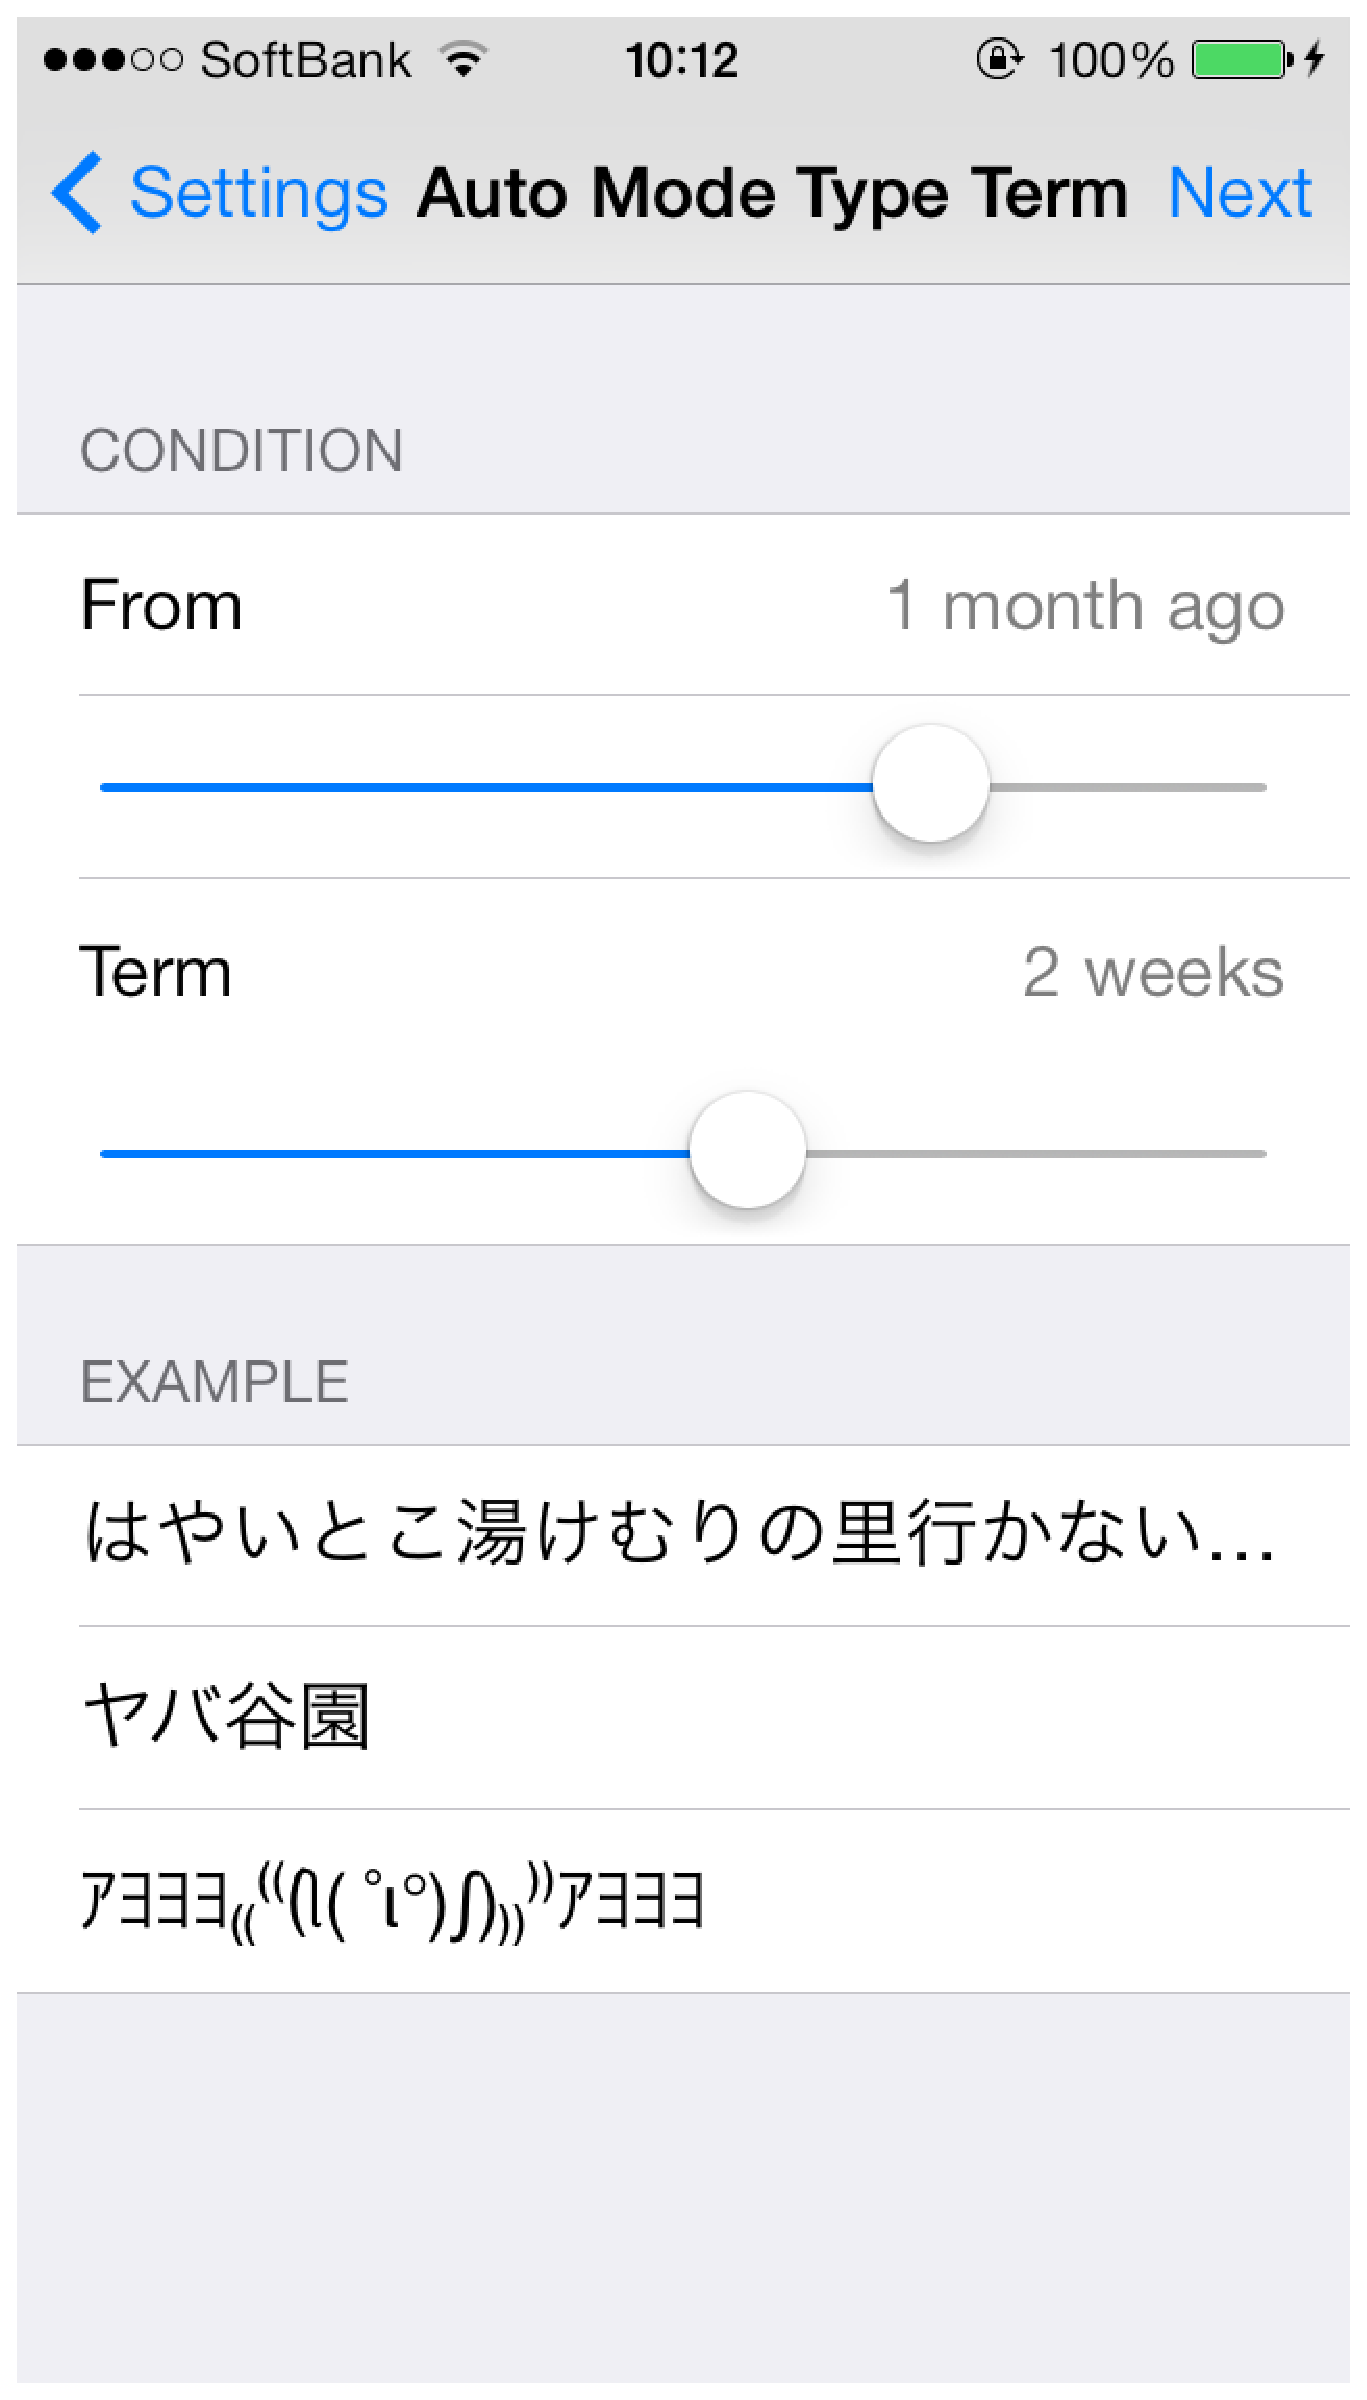
\includegraphics[width=40mm]{img/notifauthAutoTerm.eps}
    \end{center}
  \end{minipage}
  \begin{minipage}{0.49\hsize}
    \begin{center}
      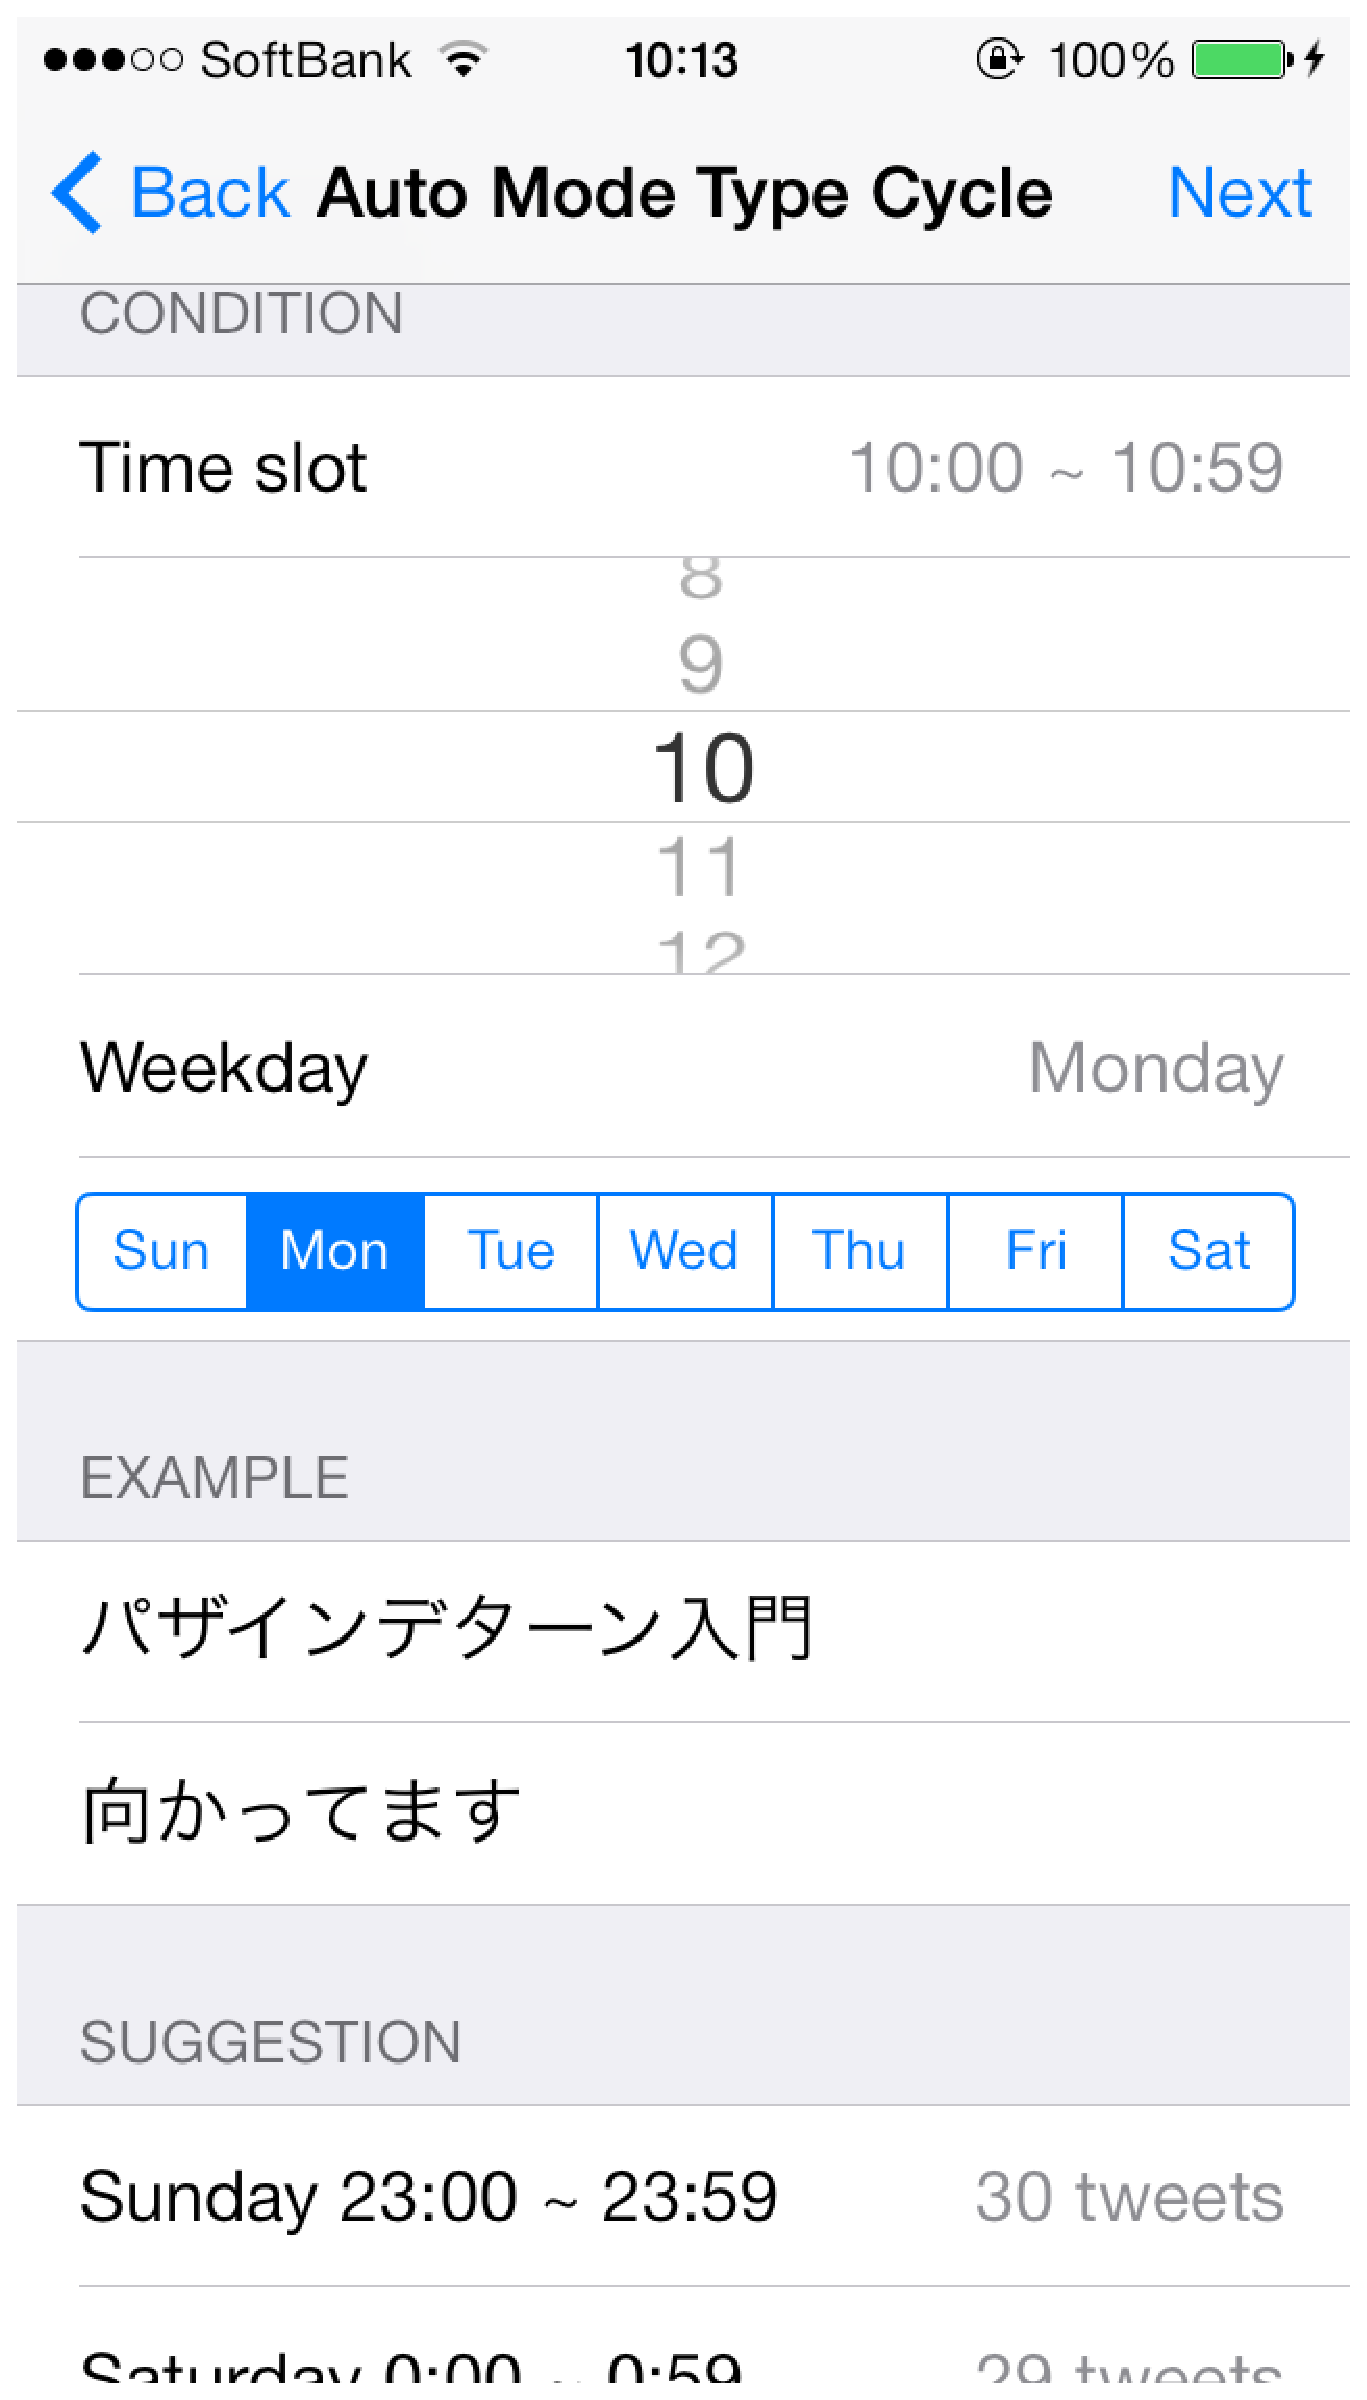
\includegraphics[width=40mm]{img/notifauthAutoCycle.eps}
    \end{center}
  \end{minipage}
  \caption{Auto Modeの2つの方式における設定画面}
  \label{notifauthSettings}
\end{figure}

\subsection{Manual Mode}
自分のツイート最新200件を取得し,その中から任意に1つ秘密情報となるものを選ぶ.
この方式では,認証時に更新分のツイートの取得を行わないため,不正解の選択肢は秘密情報を設定した時の群から選びぬかれる.
\\
\par
なお,本システムでは認証のために新たな操作を覚える負担を考慮し,認証操作に既存の携帯端末向けOSで既に実装されているロック画面中の通知機能を利用し開発を行った.
実験を行いやすくするために,iOSのロック画面を模した環境をアプリケーション内に実装した.

通知の表示画面を模した認証画面では,10個のツイートの本文と,当てはまるものがなかった場合に選択する「No match」の11つの候補を表示している.
その中から,正解だと思われるものを,指でタップし,そのまま右にスライドすることで,PINの入力画面に遷移する.

\section{実験結果}\label{result}
提案システムについて,比較のために5桁のPIN認証を追加し,それぞれの認証手法(以下,パターン)につき8日間,計32日間の実験を行った.
各パターンの実験は一つにつき8日間にわたって実施,その間に設定した日から数えて,0日目(設定直後),1日目,3日目,8日目の4回の認証試行を行った.

また,16日目が経過した段階で,2種類のパターンを比較するための中間アンケートを,32日目が経過した段階で最終アンケートを行った.
実験結果は表\ref{eachResult}に示す.

\begin{table}[ht]
  \caption{各手法における認証成功率と認証時間}
  \label{eachResult}
  \begin{center}
    \small
    \begin{tabular}{rrr}
      \bhline
      手法名 & 認証成功率(\%) & 認証時間(秒) \\ \hline
      Auto Mode Type Term & 51.79 & 22.14 \\
      Auto Mode Type Cycle & 27.59 & 22.95 \\
      Manual Mode & 94.12 & 10.74 \\
      PIN Mode & 96.08 & 2.55 \\
      \bhline
    \end{tabular}
  \end{center}
\end{table}

\section{考察}\label{discussion}
アンケートによる比較では,使いやすさと憶えやすさ両方の項目で,Manual Modeが4パターン中最も優れているとした被験者が多かった.
しかしながら,Manual Modeの認証時間はPIN Modeの4.2倍程度かかっており,特に一日に何度も認証を行う可能性の高い携帯端末では,利便性の面において改善が必要だと考えられる.

自動で設定する2手法(Auto Mode Type TermとAuto Mode Type Cycle)では,PIN認証と比べ大きく認証成功率が劣っているが,これはアンケートの内容から「設定情報は覚えているがそれに当てはまるツイートを選べない」という問題によるものだと考えられる.これを解決するために,既存手法\cite{西垣正勝:2006-03-15}で対策されているのと同様に,独立した一つの情報,本システムの場合は1ツイートに対して2〜4択で正解の選択肢を答えさせ,それを複数回繰り返すというものである.
既存手法ではこれに加え,曖昧な記憶による認証の失敗を防ぐため,はっきりと覚えている情報に対してのみ正しい回答どうかを検証した.
この2手法を導入することで,利便性と安全性について,どちらも改善できる可能性がある.
自動で設定する2手法では,定期的な秘密情報の変更を能動的に行う必要が低減されることや,時間経過によるエントロピーの増加などの利点が考えられたが,今後はそれらを活かすために認証成功率を上昇させることが最優先であると考えている.

\section{おわりに}\label{finish}
本研究では,現在の多要素認証における現状の確認,ライフログやSNSの情報を認証に使うことの有用性などを検討し,既存手法の問題点を洗いだした上で,Twitterの情報を用いた携帯端末向け個人認証の多要素化手法の提案,被験者における評価実験を実施した.

\bibliographystyle{unsrt}
\bibliography{bibtex}

\end{document}